%The document's type
\documentclass[a4paper,11pt]{article}

%Additionnal packages
\usepackage{color}
\usepackage[latin1]{inputenc}
\usepackage[T1]{fontenc}
\usepackage[english]{babel}
\usepackage{graphicx}
\usepackage{hyperref}
\usepackage{indentfirst}



%%%%%%%%%% Start TeXmacs macros
\newcommand{\tmbsl}{\ensuremath{\backslash}}
\newcommand{\tmem}[1]{{\em #1\/}}
\newcommand{\tmstrong}[1]{\textbf{#1}}
\newcommand{\tmtexttt}[1]{{\ttfamily{#1}}}
\definecolor{grey}{rgb}{0.75,0.75,0.75}
\definecolor{orange}{rgb}{1.0,0.5,0.5}
\definecolor{brown}{rgb}{0.5,0.25,0.0}
\definecolor{pink}{rgb}{1.0,0.5,0.5}
%%%%%%%%%% End TeXmacs macros

\title{Market microstructure simulation library Marketsim\\Overview}
\author{Anton Kolotaev}

\begin{document}

\maketitle

\tableofcontents



















\newpage

\section{Introduction}

Marketsim is a library for market microstructure simulation. It allows to instantiate a number of traders behaving according to various strategies and simulate their trade over number of assets. For the moment information gathered during simulation is reported in form of graphs.

This library is a result of rewriting Marketsimulator library developed in Ecole Centrale de Paris into Python. Python language was chosen as basic language for development due to its expressiveness, interactivity and availability of free high quality libraries for scientific computing. From another hand, programs in Python are not very fast and a translator from Python Marketsim object model into a C++ class templates simulation library can be developed in order to achieve maximal possible performance for simulations.

The library source can be found at \url{http://marketsimulator.svn.sourceforge.net/viewvc/marketsimulator/DevAnton/v3/}. It requires Python >= 2.6 installed. For graph plotting free \tmtexttt{Veusz} plotting software is needed (\url{http://home.gna.org/veusz/downloads/}). After installation please specify path to the Veusz executable (including executable filename) in \tmtexttt{VEUSZ\_EXE} environment variable. \tmtexttt{ArbitrageTrader} needs free \tmtexttt{blist} package to be installed: \url{http://pypi.python.org/pypi/blist/}.

\section{Discrete event simulation components}

Main class for every discrete event simulation system is a scheduler that maintains a set of actions to fulfill in future and launches them according their action times: from older ones to newer. Normally schedulers are implemented as some kind of a heap data structure in order to perform frequent operations very fast. Classical heap allows inserts into at O(logN), extracting the best element at O(logN) and accessing to the best element at O(1).

\subsection{Scheduler}

Scheduler class provides following interface:

\begin{verbatim}
class Scheduler(object):
    def reset(self)
    def currentTime(self)
    def schedule(self, actionTime, handler)
    def scheduleAfter(self, dt, handler)
    def workTill(self, limitTime)
    def advance(self, dt)
\end{verbatim}

In order to schedule an event a user should use \tmtexttt{schedule} or \tmtexttt{scheduleAfter} methods passing there an event handler which should be given as a callable object (a function, a method, lambda expression or a object exposing \tmtexttt{\_\_call\_\_} method). These functions return a callable object which can be called in order to cancel the scheduled event.

Methods \tmtexttt{workTill} and \tmtexttt{advance} advance model time calling event handlers in order of their action times. If two events have same action time it is garanteed that the event scheduled first will be executed first. These methods must not be called from an event handler. In such a case an exception will be issued.

Since a scheduler is supposed to be single for non-parallel simulations, for convenience it is made as a singleton which can be accessed via \tmtexttt{world} variable from \tmtexttt{marketsim.scheduler} module. 

\subsection{Timer}

It is a convenience class designed to represent some repeating action. It has following interface:

\begin{verbatim}
class Timer(object):
    def __init__(self, intervalFunc):
        self.on_timer = Event()
        ...
    def advise(self, listener):
        self.on_timer += listener
\end{verbatim}

It is initialized by a function defining interval of time to the next event invocation. Event handler to be invoked should be passed to \tmtexttt{advise} method (there can be plusieurs listeners).

For example, sample path a Poisson process with $\lambda$=1 can be obtained in the following way:
\begin{verbatim}
import random
from marketsim.scheduler import Timer, world

def F(timer):
    print world.currentTime
    
Timer(lambda: random.expovariate(1.)).advise(F)

world.advance(20)
\end{verbatim}

will print 

\begin{verbatim}
0.313908407622
0.795173273046
1.50151801647
3.52280681834
6.30719707516
8.48277712333
\end{verbatim}

Note that \tmtexttt{Timer} is designed to be an event source and for previous example there is a more convenient shortcut:

\begin{verbatim}
world.process(lambda: random.expovariate(1.), F)
\end{verbatim}

\section{Orders}

Traders send orders to a market. There are two basic kinds of orders: 
\begin{itemize}
\item Market orders that ask to buy or sell some asset at any price. 
\item Limit orders that ask to buy or sell some asset at price better than some limit price. If a limit order is not competely fulfilled it remains in an order book waiting to be matched with another order.
\end{itemize}
An order book processes market and limit orders but keeps persistently only limit orders. Limit orders can be cancelled by sending cancel orders.
From trader point of view there can be other order types like Iceberg order but from order book perspective it is just a sequence of basic orders: market or limit ones. 

\subsection{Basic order functionality}

Class \tmtexttt{OrderBase} provides basic functionality for market, limit and iceberg orders. It has following user interface:

\begin{verbatim}
class OrderBase(object):
    def __init__(self, volume):
        self.on_matched = Event()
        ...
    def volume(self)
    def PnL(self)
    def empty(self)
    def cancelled(self)
    def cancel(self)
    side = Side.Buy | Side.Sell
\end{verbatim}

It manages number of assets to trade (\tmtexttt{volume}), calculates P\&L for this order (positive if it is a sell order and negative if it is a buy order) and keeps a cancellation flag. An order is considered as empty if its volume is equal to 0. When order is matched (partially or completely) \tmtexttt{on\_matched} event listeners are invoked with information what order are matched, at what price and what volume with.

\subsection{Market orders}

Market orders (\tmtexttt{MarketOrderSell} and \tmtexttt{MarketOrderBuy}) derive from \tmtexttt{OrderBase} and simply add some logic how they should be processed in an order book.

Function \tmtexttt{MarketOrderT} returns factories for market orders for the given trade side:

\begin{verbatim}
def MarketOrderT(side):
    return MarketOrderSell if side==Side.Sell else MarketOrderBuy
\end{verbatim}


\subsection{Limit orders}

Limit orders (\tmtexttt{LimitOrderSell} and \tmtexttt{LimitOrderBuy}) store also their limit price and have a bit more complicated logic of processing in an order book.

Function \tmtexttt{LimitOrderT} returns factories for limit orders for the given trade side:

\begin{verbatim}
def LimitOrderT(side):
    return LimitOrderSell if side==Side.Sell else LimitOrderBuy
\end{verbatim}

\subsection{Iceberg orders}

Iceberg orders are virtual orders (so they are composed as a sequence of basic orders) and are never stored in order books. Once an iceberg order is sent to an order book, it creates an order of underlying type with volume constrained by some limit and sends it to the order book instead of itself. Once the underlying order is matched completely, the iceberg order resends another order to the order book till all iceberg order volume will be traded. 

Iceberg orders are created by the following function in curried form:

\begin{verbatim}
def iceberg(volumeLimit, orderFactory):
    def inner(*args):
        return IcebergOrder(volumeLimit, orderFactory, *args)
    return inner
\end{verbatim}

where \tmtexttt{volume} is a maximal volume of an order that can be issued by the iceberg order and \tmtexttt{orderFactory} is a factory to create underlying orders like \tmtexttt{MarketOrderSell} or \tmtexttt{LimitOrderBuy} and \tmtexttt{*args} are parameters to be passed to order's initializer.

\subsection{Cancel orders}

Cancel orders are aimed to cancel already issued limit (and possibly iceberg) orders. If a user wants to cancel an \tmtexttt{order} she should send \tmtexttt{CancelOrder(order)} to the same order book. It will notify the order book event listeners if the best order in the book has changed. Also, \tmtexttt{on\_order\_cancelled} is fired.

\subsection{Limit market orders}

Limit market order is a virtual order which is composed of a limit order and a cancel order sent immediately after the limit one thus combining behavior of market and limit orders: the trade is done at price better than given one (limit order behavior) but in case of failure the limit order is not stored in the order book (market order behavior).

\subsection{Always best orders}

Always best order is a virtual order that ensures that it has the best price in the order book. It is implemented as a limit order which is cancelled once the best price in the order queue has changed and is sent again to the order book with a price a tick better than the best price in the book. If several always best orders are sent to one side of an order book, a price race will start thus leading to their elimination by orders of the other side.

\section{Order book and order queue}

Order book represents a single asset traded in some market. Same asset traded in different markets would have different order books. Order book stores unfulfilled limit orders sent for this asset in two order queues for each trade sides (Asks for sell orders and Bids for buy orders).

Order queues are organized in a way to extract quickly the best order and place a new order inside. In order to achieve this a heap based implementation is used. 

Order book supports a notion of a tick size: all limit orders stored in the book should have prices that are multipliers of the chosen tick size. If order has a limit price not divisible by the tick size it is rounded to the closest 'weaker' tick ('floored' for buy orders and 'ceiled' for sell orders).

Market orders are processed by an order book in the following way: if there are unfulfilled limit orders at opposite trade side, the market order is matched against them till either it is fulfilled or there are no more unfilled limit orders. Price for the trade is taken as limit order limit price. Limit orders are matched in order of their price (ascending for sell orders and descending for buy orders). If two orders have the same price, it is garanteed that the elder order will be matched first.

Limit orders firstly processed exactly as market orders. If a limit order is not filled completely it is stored in a corresponding order queue.

\subsection{Order book}

Order book has following interface:

\begin{verbatim}
class OrderBook(object):
    def __init__(self, tickSize=1, label="")
    def queue(self, side)
    def tickSize(self)
    def process(self, order)
    def bids(self)
    def asks(self)
    def price(self)
    def spread(self)
\end{verbatim}

Methods \tmtexttt{bids}, \tmtexttt{asks} and \tmtexttt{queue} give access to queues composing the order book. Methods \tmtexttt{price} and \tmtexttt{spread} return middle arithmetic price and spread if they are defined (i.e. bids and asks are not empty). Orders are handled by an order book by \tmtexttt{process} method. If \tmtexttt{process} method is called recursively (e.g. from a listener of \tmtexttt{on\_best\_changed} event) its order is put into an internal queue which is to be processed when the current order processing is finished. This ensures that at every moment of time only one order is processed.

\subsection{Order queue}

Order queue has following user interface:

\begin{verbatim}
class OrderQueue(object):
    def book(self)
    def empty(self)
    def best(self)
    def withPricesBetterThan(self, limit)
    def volumeWithPriceBetterThan(self, limit)
    def sorted(self)
    def sortedPVs(self) 
\end{verbatim}

The best order in a queue can be obtained by calling \tmtexttt{best} method provided that the queue is not \tmtexttt{empty}. Method \tmtexttt{withPricesBetterThan} enumerates orders having limit price better or equal to \tmtexttt{limit}. This function is used to obtain total volume of orders that can be traded on price better or equal to the given one: \tmtexttt{volumeWithPriceBetterThan}. Property \tmtexttt{sorted} enumerates orders in their limit price order. Property \tmtexttt{sortedPVs} enumerates aggregate volumes for each price in the queue in their order.

When the best order changes in a queue (a new order arrival or the best order has matched), \tmtexttt{on\_best\_changed} event listeners get notified.

\subsection{Remote order book}

Remote book represents an order book for a remote trader. Remoteness means that there is some delay between moment when an order is sent to a market and the moment when the order is received by market so it models latency in telecommunication networks. A remote book constructor accepts a reference to an actual order book (or to another remote order book) and a reference to a two-way communication channel. Class \tmtexttt{TwoWayLink} implements a two-way telecommunication channel having different latency functions in each direction (to market and from market). 

\section{Traders}

\subsection{Basic trader functionality}

Class \tmtexttt{TraderBase} provides basic functionality for all traders: P\&L bookkeeping (\tmtexttt{PnL} method) and notifying listeners  about two events: \tmtexttt{on\_order\_sent} when a new order is sent to market and \tmtexttt{on\_traded} when an order sent to market partially or completely fulfilled.

Class \tmtexttt{SingleAssetTrader} derives from \tmtexttt{TraderBase} and adds tracking of a number of assets traded (\tmtexttt{amount} property).

\subsection{Generic one side trader}

Class \tmtexttt{OneSideTrader} derives from \tmtexttt{SingleAssetTrader} and provides generic structure for creating traders that trade only at one side. It is parametrized by following data:

\begin{itemize}
\item A book to trade in.
\item Side of the trader.
\item Event source. It is an object having \tmtexttt{advise} method that allows to start listening some events. Typical examples of event sources are timer events or an event that the best price in an order queue has changed. Of course, possible choices of event sources are not limited to these examples.
\item Function to calculate parameters of an order to create. For limit orders it should return pair \tmtexttt{(price, volume)} and for market orders it should return a 1-tuple \tmtexttt{(volume,)}. This function has one parameter - \tmtexttt{trader} which can be requested for example for its current P\&L and about the asset being traded.
\item Factory to create orders that will be used as a function in curried form \tmtexttt{side -> *orderArgs -> Order} where \tmtexttt{*orderArgs} is type of return value of the function calculating order parameters. Typical values for this factory are \tmtexttt{marketOrderT}, \tmtexttt{limitOrderT} or, for exalmple, \tmtexttt{icebergT(someVolume, limitOrderT)}.
\end{itemize}

The trader wakes up in moments of time given by the event source, calculates parameters of an order to create, creates an order and sends it to the order book.

\subsubsection{Liquidity provider}

\tmtexttt{LiquidityProvider} trader is implemented as instance of \tmtexttt{OneSideTrader}. It has followng parameters:

\begin{itemize}
\item    \tmtexttt{orderBook} - book to place orders in
\item    \tmtexttt{side} - side of orders to create (default: \tmtexttt{Side.Sell})
\item    \tmtexttt{orderFactoryT} - order factory function (default: \tmtexttt{LimitOrderT})
\item    \tmtexttt{initialValue} - initial price which is taken if \tmtexttt{orderBook} is empty (default: 100)
\item    \tmtexttt{creationIntervalDistr} - defines intervals of time between order creation 
                            (default: exponential distribution with $\lambda$=1)
\item    \tmtexttt{priceDistr} - defines multipliers for current asset price when price of order to create is calculated 
                            (default: log normal distribution with $\mu$=0 and $\sigma$=0.1)
\item    \tmtexttt{volumeDistr} - defines volumes of orders to create
                            (default: exponential distribution with $\lambda$=1)
\end{itemize}

It wakes up in moments of time given by \tmtexttt{creationIntervalDistr}, checks the last best price of orders in the corresponding queue, takes \tmtexttt{initialValue} if it is empty, multiplies it by a value taken from \tmtexttt{priceDistr} to obtain price of the order to create, calculates order volume using \tmtexttt{volumeDistr}, creates an order via \tmtexttt{orderFactoryT(side)} and sends it to the \tmtexttt{orderBook}.

\begin{figure}[htbp]
\centering
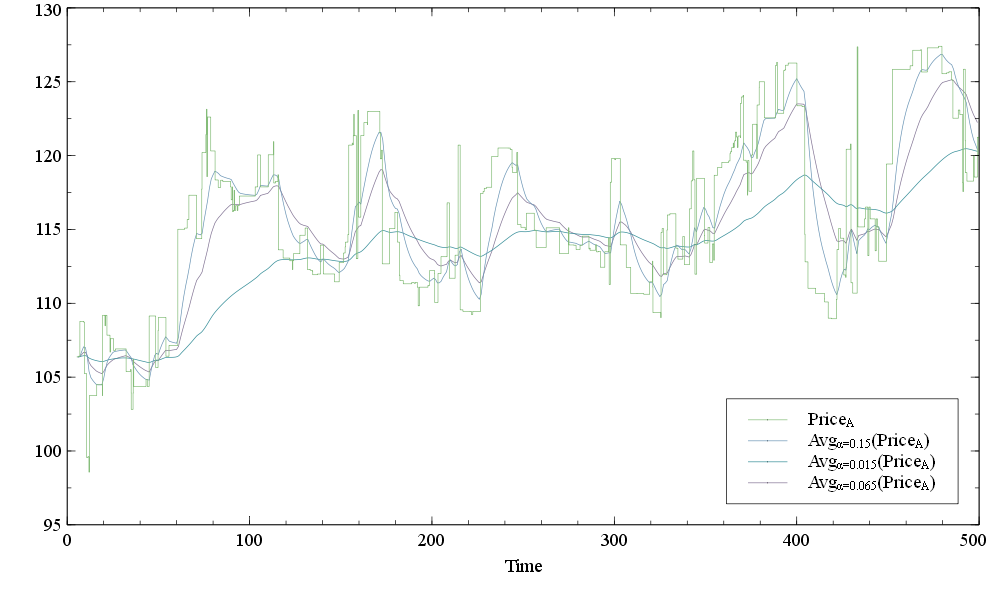
\includegraphics[width=1\linewidth]{Figures/LiquidityProvider.PNG}
\caption{Liquidity provider sample run}
\label{fig:LiquidityProvider}
\end{figure}

Sample usage:

\begin{verbatim}
from marketsim.veusz_graph import Graph, showGraphs
from marketsim.scheduler import world
from marketsim.order_queue import OrderBook
from marketsim.trader import LiquidityProvider
from marketsim.indicator import AssetPrice, avg

book_A = OrderBook(tickSize=0.01, label="A")

price_graph = Graph("Price")
 
assetPrice = AssetPrice(book_A)

price_graph.addTimeSeries([\
    assetPrice,
    avg(assetPrice, alpha=0.15),
    avg(assetPrice, alpha=0.015),
    avg(assetPrice, alpha=0.65)])

seller_A = LiquidityProvider(book_A, Side.Sell)
buyer_A = LiquidityProvider(book_A, Side.Buy)

world.workTill(500)

showGraphs("liquidity", [price_graph])
\end{verbatim}

\subsubsection{Canceller}

\tmtexttt{Canceller} is an agent aimed to cancel limit or iceberg orders issued by a trader. In order to do that it subscribes to \tmtexttt{on\_order\_sent} event of the trader, stores incoming orders in an array and in some moments of time chooses randomly an order and cancels it (In future it shall send CancelOrder to the order book).

It has following parameters:
\begin{itemize}
\item  \tmtexttt{trader} - trader to subscribe to  
\item  \tmtexttt{cancellationIntervalDistr} - intervals of times between order cancellations
                                    (default: exponential distribution with $\lambda$=1)
\item  \tmtexttt{choiceFunc} - function N -> idx that chooses which order should be cancelled
\end{itemize}

\subsection{Generic two side trader}

Class \tmtexttt{TwoSideTrader} derives from \tmtexttt{SingleAssetTrader} and provides generic structure for creating traders that trade on both sides. It is parametrized by following data (see also \tmtexttt{OneSideTrader} parameters):

\begin{itemize}
\item A book to trade in.
\item Event source. It is an object having \tmtexttt{advise} method that allows to start listening some events. 
\item Function to calculate parameters of an order to create. It should return either pair \tmtexttt{(side, *orderArgs)} if it wants to create an order, or \tmtexttt{None} if no order should be created.
\item Factory to create orders that will be used as a function in curried form \tmtexttt{side -> *orderArgs -> Order} where \tmtexttt{*orderArgs} is type of return value of the function calculating order parameters. 
\end{itemize}

The trader wakes up in moments of time given by the event source, calculates parameters and side of an order to create, if the side is defined creates an order and sends it to the order book.

\subsubsection{Fundamental value trader}

Fundamental value trader believes that an asset should cost some specific price ('fundamental value') and if current asset price is lower than fundamental value it starts to buy the asset and if the price is higher than it starts to sell the asset. \tmtexttt{FVTrader} has following parameters: 

\begin{itemize}
\item    \tmtexttt{orderBook} - book to place orders in
\item    \tmtexttt{orderFactoryT} - order factory function (default: \tmtexttt{MarketOrderT})
\item    \tmtexttt{creationIntervalDistr} - defines intervals of time between order creation 
                            (default: exponential distribution with $\lambda$=1)
\item    \tmtexttt{fundamentalValue} - defines fundamental value 
                            (default: constant 100)
\item    \tmtexttt{volumeDistr} - defines volumes of orders to create
                            (default: exponential distribution with $\lambda$=1)
\end{itemize}

\begin{figure}[htbp]
\centering
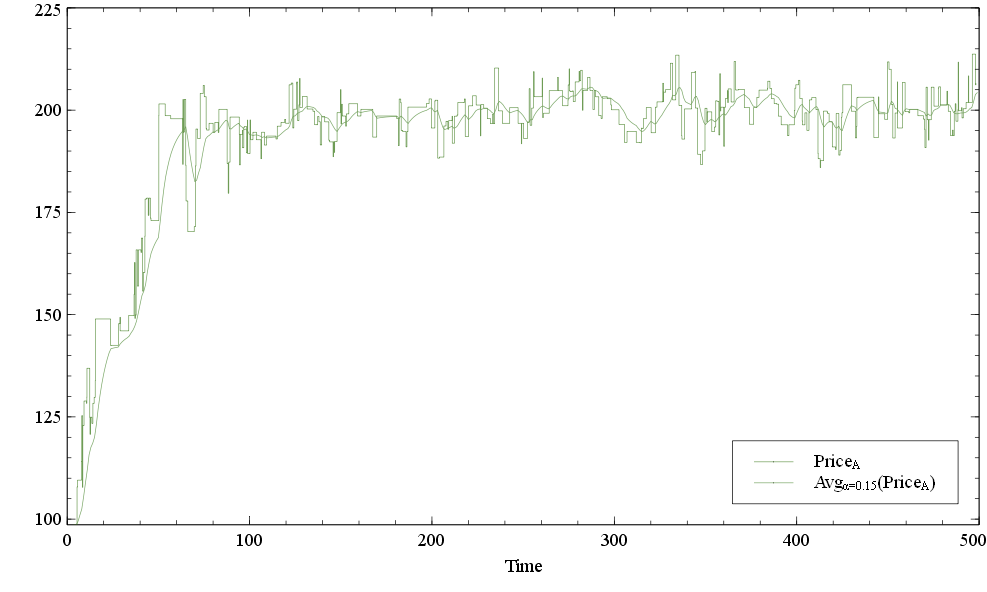
\includegraphics[width=1\linewidth]{Figures/FVTrader.PNG}
\caption{Fundamental value trader sample run (fv=200)}
\label{fig:FVTrader}
\end{figure}

Sample usage:

\begin{verbatim}
from marketsim.veusz_graph import Graph, showGraphs
from marketsim.scheduler import world
from marketsim.order_queue import OrderBook
from marketsim.trader import LiquidityProvider, FVTrader
from marketsim import Side
from marketsim.indicator import AssetPrice, avg

book_A = OrderBook(tickSize=0.01, label="A")
price_graph = Graph("Price")
 
assetPrice = AssetPrice(book_A)
price_graph.addTimeSerie(assetPrice)
price_graph.addTimeSerie(avg(assetPrice))

seller_A = LiquidityProvider(book_A, Side.Sell)
buyer_A = LiquidityProvider(book_A, Side.Buy)
trader = FVTrader(book_A, fundamentalValue=lambda: 200.)

world.workTill(500)
showGraphs("fv_trader", [price_graph])
\end{verbatim}

\subsubsection{Dependance trader}

Dependance trader believes that the fair price of an asset \textit{A} is completely correlated with price of another asset \textit{B} and the following relation should be held: \textit{$Price_{A}$ = $kPrice_B$}, where \textit{k} is some factor. It may be considered as a variety of a fundamental value trader with the exception that it is invoked every the time price of another asset \textit{B} has changed. \tmtexttt{DependanceTrader} has following parameters: 

\begin{itemize}
\item    \tmtexttt{orderBook} - book to place orders in
\item    \tmtexttt{bookToDependOn} - asset that is considered as a reference one
\item    \tmtexttt{orderFactoryT} - order factory function (default: \tmtexttt{MarketOrderT})
\item    \tmtexttt{factor} - multiplier to obtain fair asset price from the reference asset price
\item    \tmtexttt{volumeDistr} - defines volumes of orders to create
                            (default: exponential distribution with $\lambda$=1)
\end{itemize}

\begin{figure}[htbp]
\centering
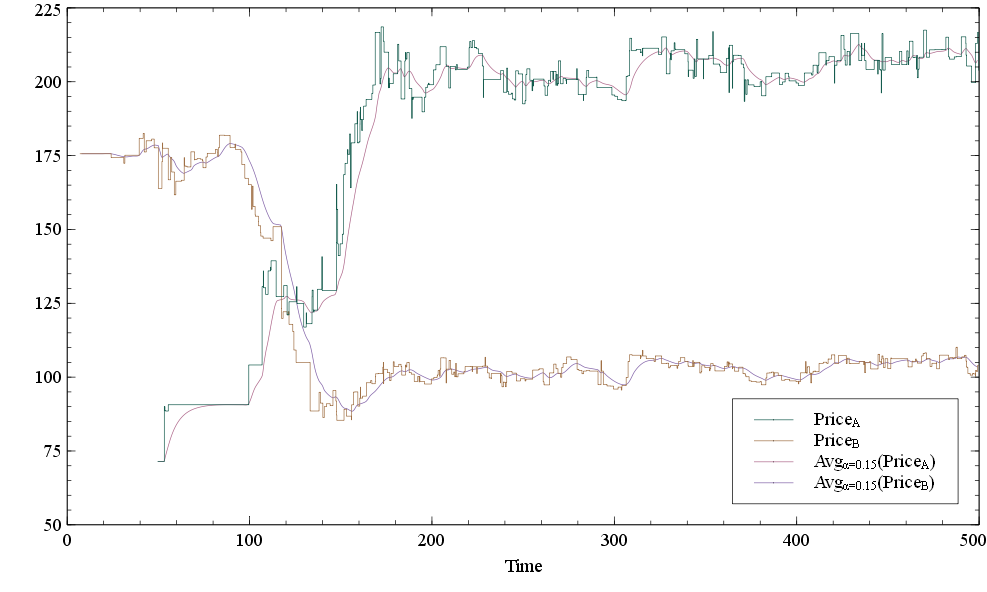
\includegraphics[width=1\linewidth]{Figures/Dependency.PNG}
\caption{Dependency trader sample run (k=0.5)}
\label{fig:Dependency}
\end{figure}

Sample usage:

\begin{verbatim}
from marketsim.veusz_graph import Graph, showGraphs
import random
from marketsim.scheduler import world
from marketsim.order_queue import OrderBook
from marketsim.trader import LiquidityProvider, DependanceTrader
from marketsim import Side
from marketsim.indicator import AssetPrice, avg

price_graph = Graph("Price")

book_A = OrderBook(tickSize=0.01, label="A")
book_B = OrderBook(tickSize=0.01, label="B")
 
assetPrice_A = AssetPrice(book_A)
price_graph.addTimeSerie(assetPrice_A)

assetPrice_B = AssetPrice(book_B)
price_graph.addTimeSerie(assetPrice_B)

price_graph.addTimeSerie(avg(assetPrice_A, alpha=0.15))
price_graph.addTimeSerie(avg(assetPrice_B, alpha=0.15))

liqVol = lambda: random.expovariate(.1)*1
seller_A = LiquidityProvider(book_A, Side.Sell, defaultValue=50., volumeDistr=liqVol)
buyer_A = LiquidityProvider(book_A, Side.Buy, defaultValue=50., volumeDistr=liqVol)

seller_B = LiquidityProvider(book_B, Side.Sell, defaultValue=150., volumeDistr=liqVol)
buyer_B = LiquidityProvider(book_B, Side.Buy, defaultValue=150., volumeDistr=liqVol)

dep_AB = DependanceTrader(book_A, book_B, factor=2)
dep_BA = DependanceTrader(book_B, book_A, factor=.5)

world.workTill(500)

showGraphs("dependency", [price_graph])
\end{verbatim}

\subsubsection{Noise trader}

Noise trader is quite dummy trader that randomly creates an order and sends it to the order book. tmtexttt{NoiseTrader} has following parameters:

\begin{itemize}
\item    \tmtexttt{orderBook} - book to place orders in
\item    \tmtexttt{orderFactoryT} - order factory function (default: \tmtexttt{MarketOrderT})
\item    \tmtexttt{creationIntervalDistr} - defines intervals of time between order creation 
                            (default: exponential distribution with $\lambda$=1)
\item    \tmtexttt{sideDistr} - side of orders to create 
                            (default: discrete uniform distribution P(Sell)=P(Buy)=.5)
\item    \tmtexttt{volumeDistr} - defines volumes of orders to create
                            (default: exponential distribution with $\lambda$=1)
\end{itemize}

\subsubsection{Signal trader}

Signal trader listens to some discrete signal and when the signal becomes more than some threshold the trader starts to buy. When the signal  gets lower than -threshold the trader starts to sell. \tmtexttt{SignalTrader} has following parameters: 

\begin{itemize}
\item    \tmtexttt{orderBook} - book to place orders in
\item    \tmtexttt{signal} - signal to be listened to
\item    \tmtexttt{orderFactoryT} - order factory function (default: \tmtexttt{MarketOrderT})
\item    \tmtexttt{threshold} - threshold when the trader starts to act (default: 0.7)
\item    \tmtexttt{volumeDistr} - defines volumes of orders to create
                            (default: exponential distribution with $\lambda$=1)
\end{itemize}

\begin{figure}[htbp]
\centering
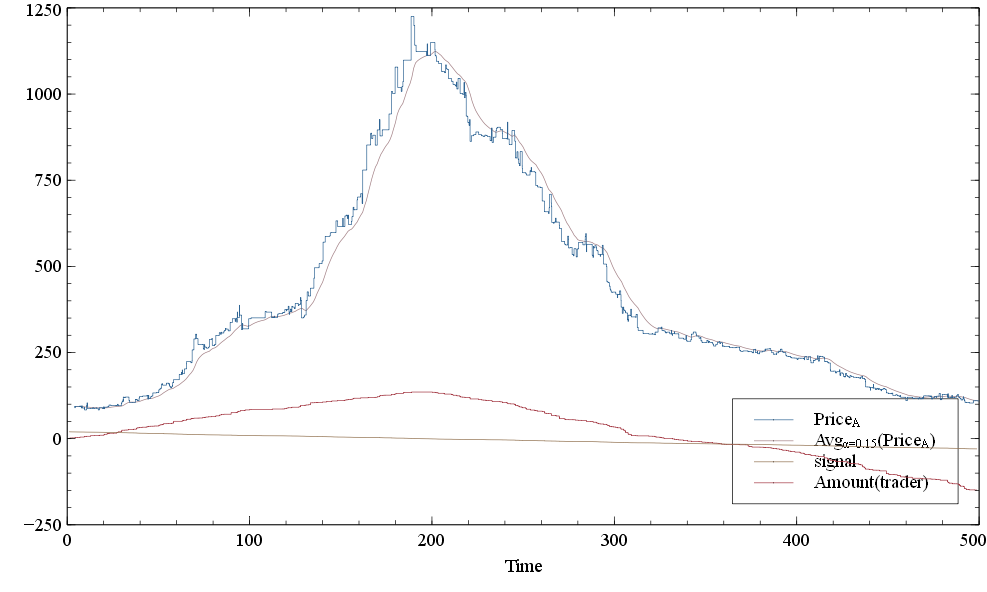
\includegraphics[width=1\linewidth]{Figures/Signal.PNG}
\caption{Signal trader sample run (signal=20-t/10)}
\label{fig:Signalr}
\end{figure}

Sample usage:

\begin{verbatim}
from marketsim.veusz_graph import Graph, showGraphs
from marketsim.scheduler import world
from marketsim.order_queue import OrderBook
from marketsim.trader import LiquidityProvider, Signal, SignalTrader
from marketsim import Side
from marketsim.indicator import AssetPrice, avg, VolumeTraded

book_A = OrderBook(tickSize=0.01, label="A")
price_graph = Graph("Price")
 
assetPrice = AssetPrice(book_A)
price_graph.addTimeSerie(assetPrice)
price_graph.addTimeSerie(avg(assetPrice))

seller_A = LiquidityProvider(book_A, Side.Sell, volumeDistr=lambda:1)
buyer_A = LiquidityProvider(book_A, Side.Buy, volumeDistr=lambda:1)
signal = Signal(initialValue=20, deltaDistr=lambda: -.1, label="signal")
trader = SignalTrader(book_A, signal)

price_graph.addTimeSerie(signal)
price_graph.addTimeSerie(VolumeTraded(trader))

world.workTill(500)
showGraphs("signal_trader", [price_graph])
\end{verbatim}

\subsubsection{Signal}

\tmtexttt{Signal} is a sample discrete signal that changes at some moments of time by incrementing on some random value. \tmtexttt{Signal} has following parameters:

\begin{itemize}
\item    \tmtexttt{initialValue} - initial value of the signal (default: 0)
\item    \tmtexttt{deltaDistr} - increment distribution function (default: normal distribution with $\mu$=0, $\sigma$=1)
\item    \tmtexttt{intervalDistr} - defines intervals of time between order creation 
                            (default: exponential distribution with $\lambda$=1)
\end{itemize}

\subsubsection{Trend follower}

Trend follower can be considered as a sort of  \tmtexttt{SignalTrader} where signal is a trend of the asset. Under trend we understand the first derivative of some moving average of asset prices. If the derivative is positive, the trader buys; if negative -- sells. Since moving average is a continuously changing signal, we check its derivative at random moments of time. \tmtexttt{TrendFollower} has following parameters: 

\begin{itemize}
\item    \tmtexttt{orderBook} - book to place orders in
\item    \tmtexttt{average} - moving average object. It should have methods \tmtexttt{update(time,value)} and \tmtexttt{derivativeAt(time)}. By default, we use exponentially weighted moving average with $\alpha=0.15$.
\item    \tmtexttt{orderFactoryT} - order factory function (default: \tmtexttt{MarketOrderT})
\item    \tmtexttt{threshold} - threshold when the trader starts to act (default: 0.)
\item    \tmtexttt{creationIntervalDistr} - defines intervals of time between order creation 
                            (default: exponential distribution with $\lambda$=1)
\item    \tmtexttt{volumeDistr} - defines volumes of orders to create
                            (default: exponential distribution with $\lambda$=1)
\end{itemize}

\subsection{Arbitrage trader}

Arbitrage trader tries to make arbitrage trading the same asset on different markets. Once a bid price at one market becomes more than ask price at other market, the trader sends two complimentary market orders with opposite sides and the same volume (which is calculated using order queue's \tmtexttt{volumeWithPriceBetterThan} method) having thus non-negative profit. \tmtexttt{ArbitrageTrader} is initialized by a sequence of order books it will follow for.

\begin{figure}[htbp]
\centering
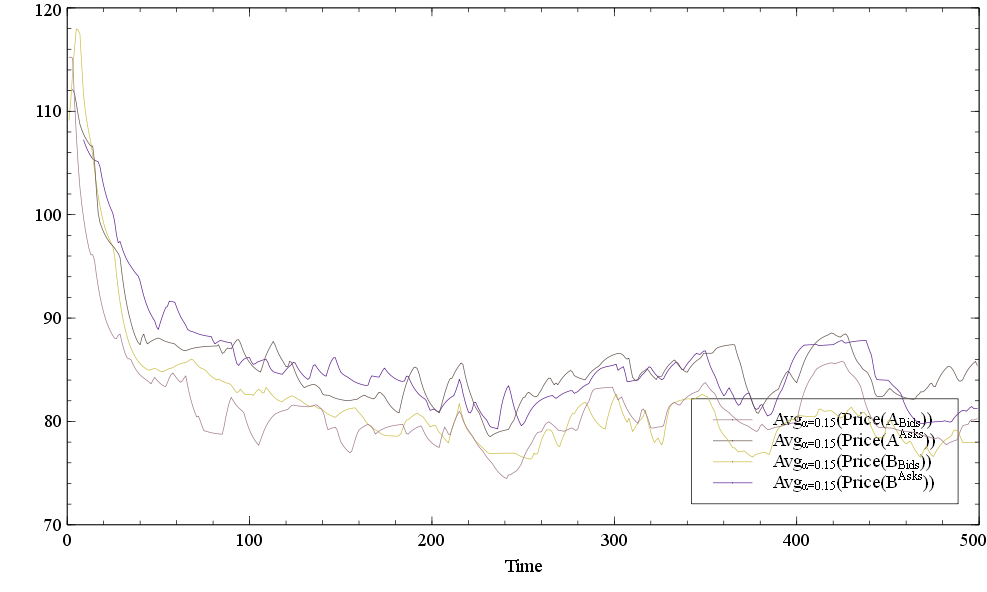
\includegraphics[width=1\linewidth]{Figures/Arbitrage_Bid_Ask_Spread.PNG}
\caption{Arbitrage trader sample run (Bid/Ask price)}
\label{fig:ArbBidAsk}
\end{figure}

\begin{figure}[htbp]
\centering
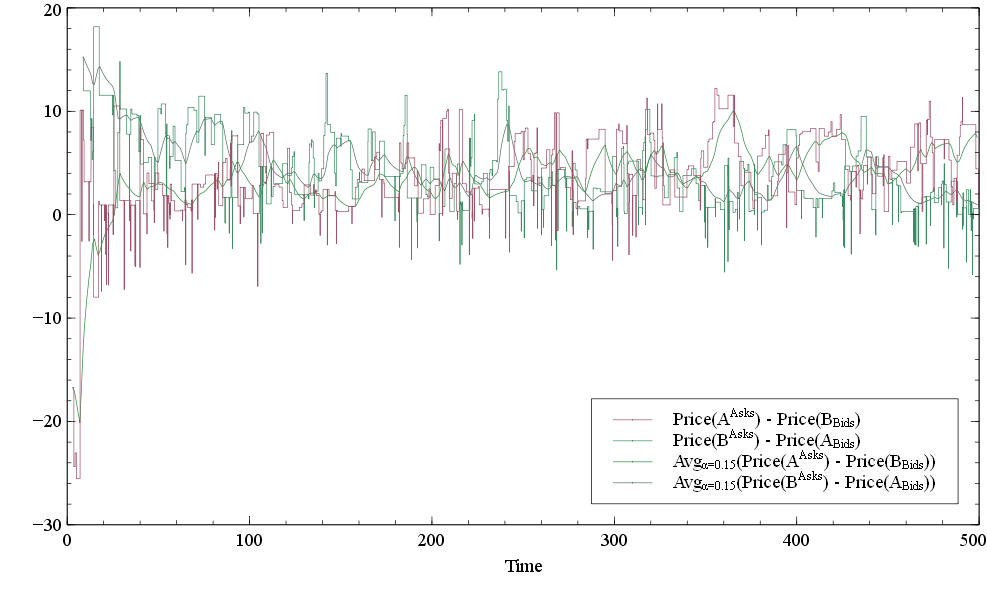
\includegraphics[width=1\linewidth]{Figures/Arbitrage_Cross_Spread.PNG}
\caption{Arbitrage trader sample run (Cross spread)}
\label{fig:ArbCross}
\end{figure}

Sample usage:

\begin{verbatim}
from marketsim.veusz_graph import Graph, showGraphs
from marketsim.scheduler import world
from marketsim.order_queue import OrderBook
from marketsim.trader import LiquidityProvider
from marketsim.arbitrage_trader import ArbitrageTrader
from marketsim import Side
from marketsim.indicator import AssetPrice, avg, CrossSpread

book_A = OrderBook(tickSize=0.01, label="A")
book_B = OrderBook(tickSize=0.01, label="B")

spread_graph = Graph("Bid-Ask Spread")
cross_graph = Graph("Cross Bid-Ask Spread")

cross_AB = CrossSpread(book_A, book_B)
cross_BA = CrossSpread(book_B, book_A)
cross_graph.addTimeSerie(cross_AB)
cross_graph.addTimeSerie(cross_BA)
cross_graph.addTimeSerie(avg(cross_AB))
cross_graph.addTimeSerie(avg(cross_BA))

spread_graph.addTimeSerie(avg(BidPrice(book_A)))
spread_graph.addTimeSerie(avg(AskPrice(book_A)))
spread_graph.addTimeSerie(avg(BidPrice(book_B)))
spread_graph.addTimeSerie(avg(AskPrice(book_B)))

seller_A = LiquidityProvider(book_A, Side.Sell)
buyer_A = LiquidityProvider(book_A, Side.Buy)

seller_B = LiquidityProvider(book_B, Side.Sell)
buyer_B = LiquidityProvider(book_B, Side.Buy)

arbitrager = ArbitrageTrader(book_A, book_B)

world.workTill(500)

showGraphs("arbitrage", [spread_graph, cross_graph])
\end{verbatim}
\end{document}





